\subsection{Calibration and power results}
Table~\ref{tab:nullnew} reports null FWER for the common minor-plus-joint-rank projection. Exact methods have their finite-sample guarantee; the multiplier methods are evaluated empirically. All cellwise Wilson intervals, simultaneous coverage outcomes and replication records accompany the article.
\begin{table}[htbp]\centering\small
\setlength{\tabcolsep}{4pt}
\caption{False-order FWER at nominal 0.05; 1,000 datasets in each null cell. P: one-matching exact; M8: merged p-values; E8/E64: evidence aggregation over 8/64 matchings; M-C: multiplier contrasts; M-B: multiplier rectangle. Both Hoeffding controls have zero false orders in these cells. All methods use the local family.}\label{tab:nullnew}
\begin{lrbox}{\resultsbox}\begin{tabular}{lrrrrrr}
\toprule
Model, $p$, $n$ & P & M8 & E8 & E64 & M-C & M-B\\
\midrule
Gaussian null, 12, 252 & 0.024 & 0.000 & 0.000 & 0.001 & 0.072 & 0.002\\
Gaussian null, 12, 1008 & 0.029 & 0.000 & 0.000 & 0.000 & 0.062 & 0.003\\
Gaussian null, 12, 4096 & 0.032 & 0.000 & 0.001 & 0.000 & 0.042 & 0.001\\
Discrete null, 12, 1008 & 0.029 & 0.000 & 0.001 & 0.000 & 0.050 & 0.001\\
Gaussian null, 52, 1008 & 0.035 & 0.000 & 0.000 & 0.000 & 0.077 & 0.000\\
\bottomrule\end{tabular}\end{lrbox}\ifdim\wd\resultsbox>\linewidth\resizebox{\linewidth}{!}{\usebox{\resultsbox}}\else\usebox{\resultsbox}\fi\end{table}
The largest one-matching null estimate is 0.035, with an individual Wilson interval [0.025,0.048] (Gaussian null, $p=52$, $n=1008$). This is a cellwise Monte Carlo summary; simultaneous calibration is established by the exact-test argument.
\begin{table}[htbp]\centering\small
\setlength{\tabcolsep}{4pt}
\caption{Probability of declaring the true unique hub using the same minor and joint-rank projection. Local comparisons; 200 repetitions for the displayed $p=12$ star cells and 100 for $p=52$. Both Hoeffding controls declare no unique hub in these star cells; full results are archived. Path projection is evaluated separately on paired subsets.}\label{tab:powernew}
\begin{lrbox}{\resultsbox}\begin{tabular}{lrrrrrr}
\toprule
Model, $p$, $n$ & P & M8 & E8 & E64 & M-C & M-B\\
\midrule
Gaussian star, 12, 1008 & 0.000 & 0.000 & 0.000 & 0.000 & 1.000 & 0.900\\
Gaussian star, 12, 4096 & 1.000 & 0.990 & 1.000 & 1.000 & 1.000 & 1.000\\
$t_5$ star, 12, 1008 & 0.000 & 0.000 & 0.000 & 0.000 & 1.000 & 0.195\\
$t_5$ star, 12, 4096 & 1.000 & 1.000 & 1.000 & 1.000 & 1.000 & 1.000\\
Gaussian star, 52, 4096 & 0.670 & 0.000 & 1.000 & 1.000 & 1.000 & 1.000\\
$t_5$ star, 52, 4096 & 0.720 & 0.000 & 1.000 & 1.000 & 1.000 & 1.000\\
Near-tie star, 12, 4096 & 0.000 & 0.000 & 0.000 & 0.000 & 0.000 & 0.000\\
Near-tie star, 52, 4096 & 0.000 & 0.000 & 0.000 & 0.000 & 0.000 & 0.000\\
\bottomrule\end{tabular}\end{lrbox}\ifdim\wd\resultsbox>\linewidth\resizebox{\linewidth}{!}{\usebox{\resultsbox}}\else\usebox{\resultsbox}\fi\end{table}
Power is interpreted jointly with FWER. The multiplier contrast procedure exceeds nominal error in some IID null cells; higher declaration rates in those regimes do not establish valid superiority. The exact evidence methods provide a comparison whose error guarantee does not rely on the Gaussian approximation.
Figure~\ref{fig:powernew} compares the full sample-size grids. The merged rule is assessed as an exact alternative, rather than assumed to recover U-statistic efficiency. The bounded-range U-statistic comparator shows whether using all pairs alone is sufficient; the matched multiplier rectangle and contrast procedures isolate the effect of shared-edge covariance and direct calibration.
\begin{figure}[htbp]\centering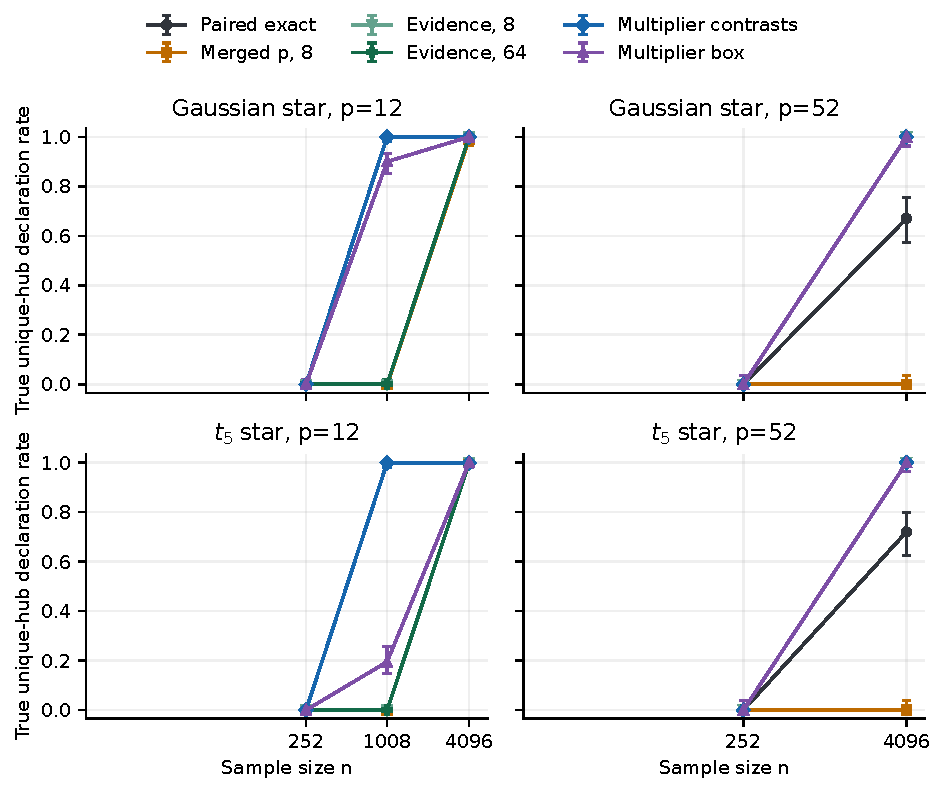
\includegraphics[width=\textwidth]{Fig_comparative.pdf}
\caption{Unique-hub declarations under the common joint projection. Curves use matched data; intervals are individual 95\% Wilson Monte Carlo intervals. All specified sample sizes and both separated distributions are shown.}\label{fig:powernew}\end{figure}
\subsection{Projection ablation}
\begin{table}[htbp]\centering\small
\setlength{\tabcolsep}{4pt}
\caption{Paired projection ablation at $p=12,n=1008$, using the same first 100 datasets per cell. Degree widths compare the minor with path LP. Rank widths compare marginal, joint pair/conservation and path projection. Complete results for all eight tests and sizes are archived. Width is upper minus lower endpoint.}\label{tab:ablation}
\begin{lrbox}{\resultsbox}\begin{tabular}{llrrrrr}
\toprule
Model & Test & $W_d$ minor & $W_d$ path & $W_r$ marg. & $W_r$ joint & $W_r$ path\\
\midrule
Gaussian star & P & 8.94 & 8.40 & 11.00 & 11.00 & 11.00\\
Gaussian star & E64 & 9.02 & 8.33 & 11.00 & 11.00 & 11.00\\
Gaussian star & M-C & 0.00 & 0.00 & 9.17 & 9.17 & 9.17\\
Near-tie star & P & 9.92 & 9.45 & 11.00 & 11.00 & 11.00\\
Near-tie star & E64 & 9.99 & 9.51 & 11.00 & 11.00 & 11.00\\
Near-tie star & M-C & 3.93 & 3.54 & 11.00 & 10.90 & 10.81\\
Chain & P & 8.00 & 4.58 & 11.00 & 11.00 & 11.00\\
Chain & E64 & 6.477 & 3.968 & 11.00 & 10.99 & 10.99\\
Chain & M-C & 0.00 & 0.00 & 7.67 & 7.67 & 7.67\\
Two hubs & P & 8.43 & 6.66 & 11.00 & 10.96 & 10.96\\
Two hubs & E64 & 5.82 & 5.11 & 10.98 & 10.54 & 10.54\\
Two hubs & M-C & 0.58 & 0.58 & 7.67 & 7.67 & 7.67\\
\bottomrule\end{tabular}\end{lrbox}\ifdim\wd\resultsbox>\linewidth\resizebox{\linewidth}{!}{\usebox{\resultsbox}}\else\usebox{\resultsbox}\fi\end{table}
Table~\ref{tab:ablation} locates the path-projection gain mainly in degree precision. For one-matching inference, Gaussian-star mean degree width decreases from 8.94 to 8.40; in the chain it decreases from 8.00 to 4.58. The corresponding E64 chain widths decrease from 6.477 to 3.968. Most exact rank widths remain approximately 11, the full-range width at $p=12$. In the near-tie multiplier example, the path stage decreases mean rank width only from 10.90 to 10.81. Thus these $n=1008$ simulations demonstrate useful degree restrictions but little additional rank resolution: tighter degree bounds need not establish a positive degree difference between two vertices.

Population degree ties also impose an irreducible rank width. Even with the exact Gaussian-star tree known, its eleven leaves occupy ranks 2--12 under the tie-inclusive target, giving mean rank width $110/12=9.17$. For the chain and two-hub trees, the corresponding mean is $92/12=7.67$. The displayed multiplier results at these widths therefore retain the required tied ranks. Degree-conservation and direct-pair rank outputs are archived separately from the path stage.

Across all sample sizes and methods in the $p=12$ simulation path stage{,} the local family accounts for 950{,}820 LP objectives and 375{,}946 independently verified improving rational certificates. The complete family adds 913{,}068 objectives and 273{,}901 certificates. The totals across both families are therefore 1{,}863{,}888 LP objectives and 649{,}847 certificates. These totals include all evaluated path-stage cells{,} rather than only the subset displayed in Table~\ref{tab:ablation}.
\subsection{Comparison-family ablation}
\begin{table}[htbp]\centering\small
\setlength{\tabcolsep}{4pt}
\caption{Matched local/complete family ablation at $p=12,n=4096$, 100 datasets per cell. Closed-order counts use the same $m(m-1)$ potential ordered pairs in either family. More tested comparisons also incur a larger multiplicity penalty.}\label{tab:family}
\begin{lrbox}{\resultsbox}\begin{tabular}{llrrrrrr}
\toprule
Model & Test & Orders L & Orders A & $W_d$ L & $W_d$ A & $W_r$ L & $W_r$ A\\
\midrule
Gaussian star & P & 113.0 & 530.7 & 0.14 & 0.25 & 9.17 & 9.17\\
Gaussian star & E64 & 110.8 & 579.0 & 0.00 & 0.00 & 9.17 & 9.17\\
Gaussian star & M-C & 214.4 & 643.0 & 0.00 & 0.00 & 9.17 & 9.17\\
$t_5$ star & P & 112.0 & 527.8 & 0.17 & 0.31 & 9.17 & 9.17\\
$t_5$ star & E64 & 110.5 & 573.7 & 0.00 & 0.00 & 9.17 & 9.17\\
$t_5$ star & M-C & 193.3 & 629.0 & 0.00 & 0.00 & 9.17 & 9.17\\
Near-tie star & P & 137.3 & 331.6 & 6.40 & 7.20 & 11.00 & 11.00\\
Near-tie star & E64 & 170.8 & 393.1 & 5.53 & 6.54 & 10.99 & 11.00\\
Near-tie star & M-C & 331.1 & 969.4 & 1.66 & 1.67 & 10.16 & 10.17\\
Chain & P & 850.2 & 1338.6 & 0.14 & 0.00 & 7.98 & 7.67\\
Chain & E64 & 923.0 & 1396.0 & 0.00 & 0.00 & 7.67 & 7.67\\
Chain & M-C & 1374.2 & 1766.2 & 0.00 & 0.00 & 7.67 & 7.67\\
Two hubs & P & 624.1 & 1117.3 & 0.99 & 0.38 & 7.67 & 7.67\\
Two hubs & E64 & 659.5 & 1157.1 & 0.97 & 0.02 & 7.67 & 7.67\\
Two hubs & M-C & 725.3 & 1538.1 & 0.00 & 0.00 & 7.67 & 7.67\\
\bottomrule\end{tabular}\end{lrbox}\ifdim\wd\resultsbox>\linewidth\resizebox{\linewidth}{!}{\usebox{\resultsbox}}\else\usebox{\resultsbox}\fi\end{table}
Table~\ref{tab:family} shows a model-dependent trade-off. For one-matching inference in the Gaussian star, complete comparisons increase mean degree width from 0.14 to 0.25 despite increasing the closed-order count from 113.0 to 530.7. In the near-tie E64 example, width increases from 5.53 to 6.54. Conversely, complete comparisons improve the one-matching chain width from 0.14 to 0.00 and the two-hub width from 0.99 to 0.38; for E64 in the two-hub model they reduce it from 0.97 to 0.02.

The procedures recalibrate their tested families, so their rejected-order relations need not be nested. At $p=12$, the local and complete families contain 1,320 and 4,290 ordered hypotheses. For the Holm methods, the first threshold decreases from $0.05/1320$ to $0.05/4290$; multiplier contrasts also recalibrate a larger maximum. This can remove weak local comparisons important to screening incident hub edges, while adding many nonlocal orders. The number of certified orders alone therefore does not determine degree resolution. Holding one valid relation fixed and adding further valid comparisons can only tighten exact bounds over the resulting outer family; changing the calibrated relation is a different comparison. Complete testing is useful when its additional tree restrictions outweigh its multiplicity cost, as in the chain and two-hub examples.
\subsection{Frequency-reference results}
\begin{table}[H]\centering\small
\setlength{\tabcolsep}{4pt}
\caption{Practical row-bootstrap frequency rule on matched Gaussian samples, $p=12$, 499 draws. Hub declarations require unique-hub frequency at least 0.95; edge declarations require selection frequency at least 0.95. False edge declarations are familywise events. Frequencies have no general confidence guarantee.}\label{tab:frequency}
\begin{lrbox}{\resultsbox}\begin{tabular}{lrrrrr}
\toprule
Model & $n$ & $R$ & True hub & False hub & False edge\\
\midrule
Gaussian star & 1008 & 200 & 1.000 & 0.000 & 0.000\\
Gaussian star & 4096 & 200 & 1.000 & 0.000 & 0.000\\
Gaussian null & 1008 & 1000 & -- & 0.000 & 0.043\\
Gaussian null & 4096 & 1000 & -- & 0.000 & 0.049\\
Near-tie star & 1008 & 200 & 0.020 & 0.000 & 0.220\\
Near-tie star & 4096 & 200 & 0.060 & 0.000 & 0.225\\
\bottomrule\end{tabular}\end{lrbox}\ifdim\wd\resultsbox>\linewidth\resizebox{\linewidth}{!}{\usebox{\resultsbox}}\else\usebox{\resultsbox}\fi\end{table}
The frequency reference targets estimated-tree stability. Under the Gaussian null every edge can occur in an optimal population tree, but none is necessary and no vertex is a population unique hub. A high-frequency edge declaration is therefore counted as false necessity in that setting. This definition avoids interpreting frequent selection as a simultaneous population certificate.
